% Placee APRES les sections de simulation : elle confronte le modele des
% sections 12-14 aux mesures de la section 11.
\section{Comparing the Simulation with the Measurement}
\label{sec:comparison}

The script \texttt{unified\_filament\_slider\_v3.py} implements both directions of the link between the simulation and a real interferometric measurement, so that the two can be compared directly.

On the experimental side, \texttt{find\_1storder\_peak} locates the side band of a raw interferogram in Fourier space by masking out the central DC region and searching for the strongest remaining peak, implementing the Takeda demodulation step described above. \texttt{reconstruct} then crops a disk of radius set by the numerical aperture around that peak and inverse transforms it back to real space, giving the complex field $c(x,y)$ from which the phase is extracted. \texttt{fit\_plane\_from\_mask}, applied over user selected background regions through \texttt{baseline\_rects\_to\_mask}, removes any residual linear phase tilt from small optical misalignments that the reference division does not fully cancel, exactly the correction motivated at the end of the phase retrieval derivation above. \texttt{preprocess\_side\_full} chains these steps into the full pipeline from a raw pair of interferograms, signal and reference, to a clean two dimensional phase map.

On the simulation side, \texttt{build\_abel\_matrix} discretizes the forward Abel transform directly as a matrix acting on the non uniform radial grid produced by the QDHT, using the exact shell integral of $r/\sqrt{r^2-x^2}$ over each radial bin rather than a naive trapezoidal sum on that grid, so that the same physical relation $F(x)=2\int_x^\infty f(r)r\,dr/\sqrt{r^2-x^2}$ used above for the inversion is applied here in the forward direction. \texttt{abel\_phase\_2d} assembles the total refractive index change $\Delta n$ from every channel the propagation code tracks, the Drude plasma contribution from the free electron density, the Lorentz contribution from the self-trapped exciton density, the Kerr contribution from the local intensity, and a thermal contribution computed by \texttt{precompute\_dn\_thermal} from the energy deposited by trapped carriers relaxing into phonons, before applying the Abel matrix to predict the phase map a real interferometer would record for that simulated filament at a given experimental probe delay.

\begin{figure}[htbp]
    \centering
    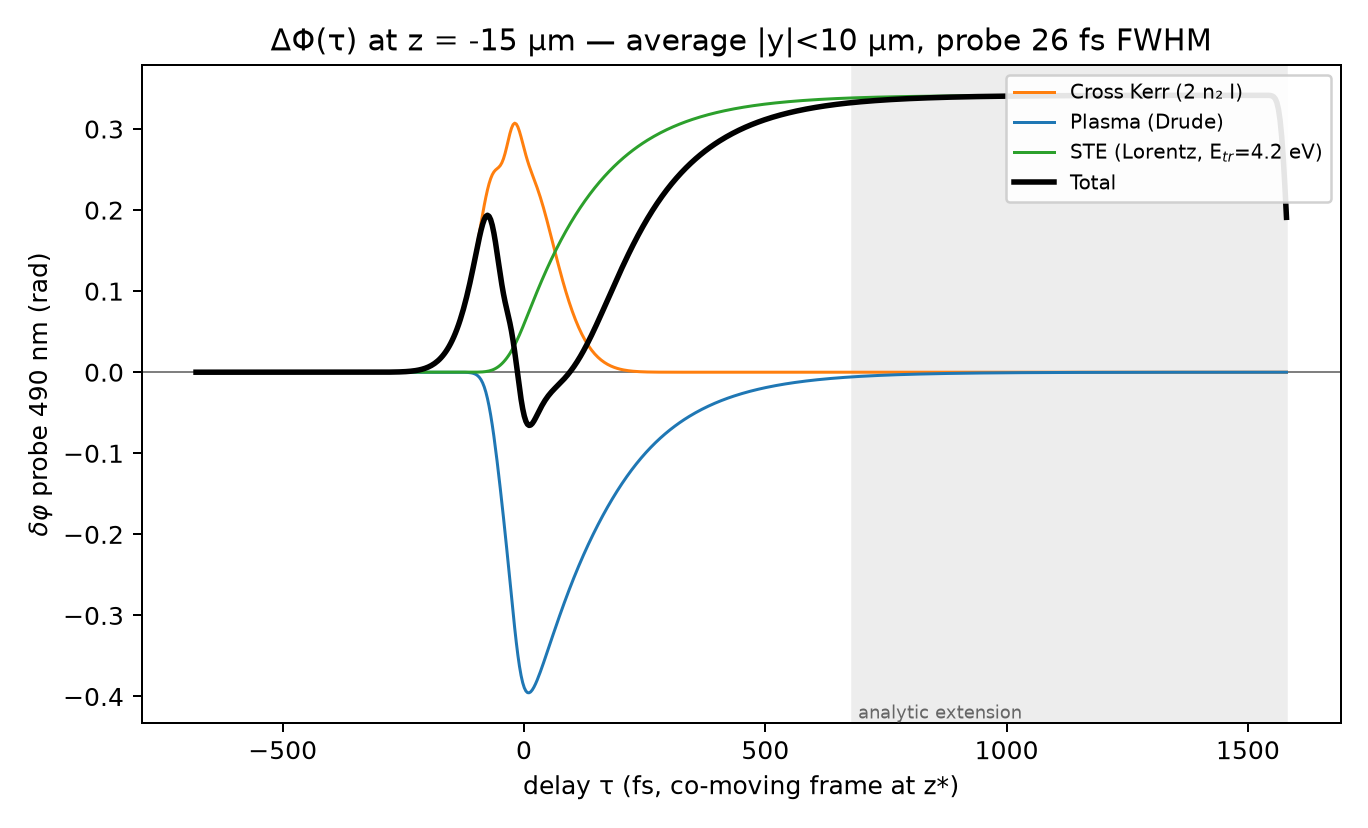
\includegraphics[width=0.85\linewidth]{fig10_dephasage.png}
    \caption{Predicted probe phase shift $\delta\varphi(\tau)$ at $490\ \text{nm}$ at the nonlinear focus, decomposed into its three channels (cross-Kerr, Drude plasma, bound STE) and their sum, convolved with a $26\ \text{fs}$ probe pulse. The sequence reproduces the qualitative structure reported by Mouskeftaras et al.~\cite{mouskeftaras2012} for single-pulse pump-probe interferometry in $\mathrm{SiO}_2$: an initial positive Kerr phase synchronous with the pump, an abrupt swing to negative as free carriers appear, and a delayed recovery to a positive plateau as trapping converts $N$ into $N_{STE}$. The comparable magnitude of the Kerr and plasma contributions here, rather than Kerr dominating as in that reference, is expected given the different regime: this trace is taken at the filamentation clamping intensity, where $n_2I\approx N/(2\rho_c)$ by construction (Section~\ref{sec:filamentation}), whereas the cited measurement was made well below threshold.}
    \label{fig:fig10_dephasage}
\end{figure}

\authornote{The thermal channel in \texttt{precompute\_dn\_thermal} assumes isochoric heating with a single phonon relaxation time \texttt{tau\_ph\_fs} and a fixed deposited energy per trapped carrier. I have not verified this against a reference for the thermo-optic coefficient $dn/dT$ or the heat capacity values used. If you can point me to the source for these, I will add the derivation and the citation here.}
